\documentclass[border=12pt]{standalone}
\usepackage{tikz}
\usetikzlibrary{arrows.meta, positioning, calc, fit, decorations.pathreplacing}

\begin{document}
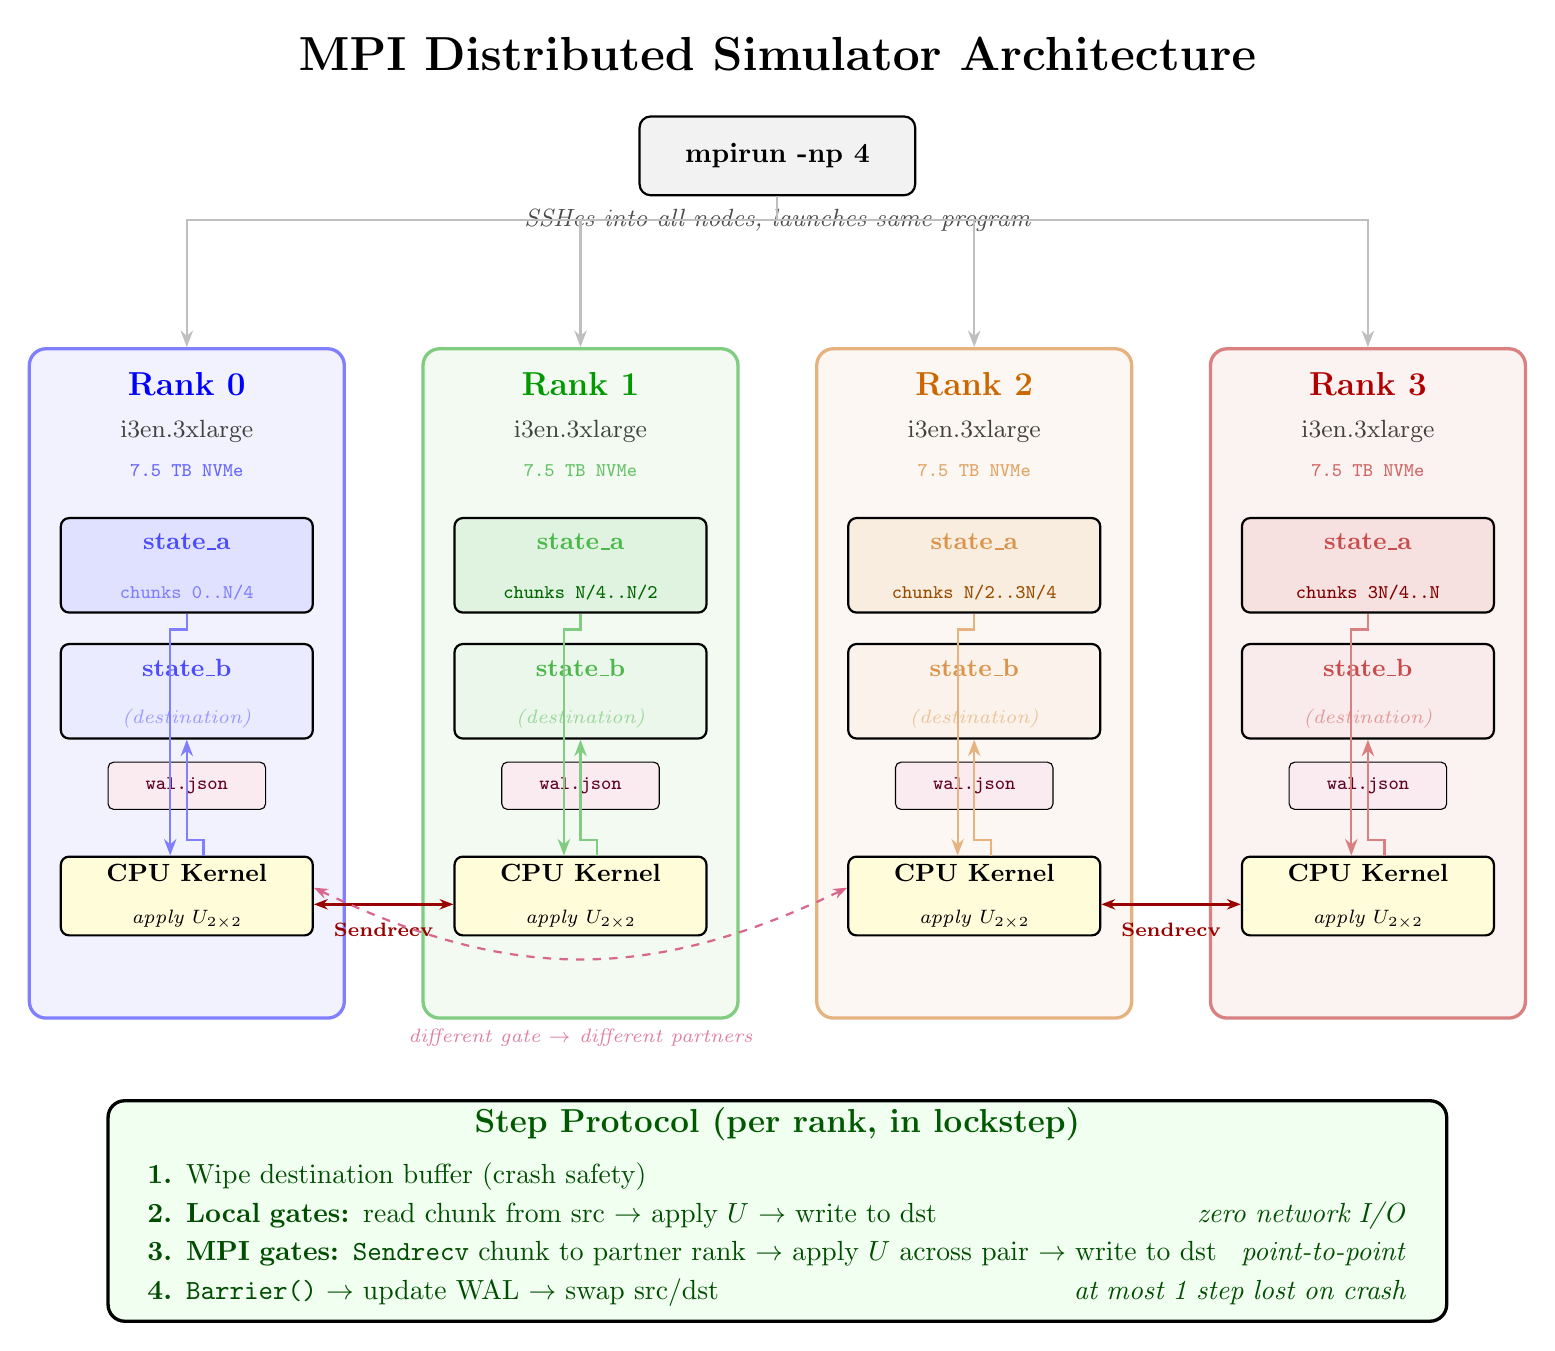
\begin{tikzpicture}[
    myarrow/.style={-{Stealth[length=6pt]}, thick},
    biarrow/.style={{Stealth[length=5pt]}-{Stealth[length=5pt]}, thick},
    heading/.style={font=\LARGE\bfseries},
    note/.style={font=\small\itshape, text=gray!60!black},
]

% ===================== TITLE =====================
\node[heading] at (9, 16.5) {MPI Distributed Simulator Architecture};

% ===================== LAUNCH =====================
\node[draw, thick, fill=gray!10, rounded corners=4pt,
      minimum width=3.5cm, minimum height=1cm,
      font=\normalsize\bfseries] (launch) at (9, 15.2)
    {mpirun -np 4};
\node[note, below=1pt of launch] {SSHes into all nodes, launches same program};

% ===================== 4 RANKS =====================
% Each rank is a box with: NVMe storage, CPU, state_a/b, WAL

\foreach \r/\x/\col in {0/1.5/blue, 1/6.5/green!60!black, 2/11.5/orange!80!black, 3/16.5/red!70!black} {

    % Main node box
    \node[draw, very thick, fill=\col!5, rounded corners=6pt,
          minimum width=4cm, minimum height=8.5cm,
          draw=\col!50] (rank\r) at (\x, 8.5) {};

    % Title
    \node[font=\large\bfseries, text=\col] at (\x, 12.3)
        {Rank \r};
    \node[font=\small, text=gray!50!black] at (\x, 11.7)
        {i3en.3xlarge};

    % NVMe label
    \node[font=\scriptsize\ttfamily, text=\col!60] at (\x, 11.2)
        {7.5 TB NVMe};

    % state_a box
    \node[draw, thick, fill=\col!12, rounded corners=3pt,
          minimum width=3.2cm, minimum height=1.2cm] (sa\r) at (\x, 10.0) {};
    \node[font=\small\bfseries, text=\col!70] at (\x, 10.3) {state\_a};

    % state_b box
    \node[draw, thick, fill=\col!8, rounded corners=3pt,
          minimum width=3.2cm, minimum height=1.2cm] (sb\r) at (\x, 8.4) {};
    \node[font=\small\bfseries, text=\col!70] at (\x, 8.7) {state\_b};
    \node[font=\scriptsize\itshape, text=\col!40] at (\x, 8.05) {(destination)};

    % WAL
    \node[draw, thin, fill=purple!8, rounded corners=2pt,
          minimum width=2cm, minimum height=0.6cm,
          font=\scriptsize\ttfamily, text=purple!50!black] (wal\r) at (\x, 7.2)
        {wal.json};

    % CPU kernel
    \node[draw, thick, fill=yellow!15, rounded corners=3pt,
          minimum width=3.2cm, minimum height=1cm] (cpu\r) at (\x, 5.8) {};
    \node[font=\small\bfseries] at (\x, 6.1) {CPU Kernel};
    \node[font=\scriptsize\itshape] at (\x, 5.5) {apply $U_{2\times 2}$};

    % Arrow: launch -> rank
    \draw[myarrow, gray!50] (launch.south) -- ++(0, -0.3) -| (rank\r.north);
}

% Fix chunk labels properly
\node[font=\scriptsize\ttfamily, text=blue!50] at (1.5, 9.65) {chunks 0..N/4};
\node[font=\scriptsize\ttfamily, text=green!40!black] at (6.5, 9.65) {chunks N/4..N/2};
\node[font=\scriptsize\ttfamily, text=orange!60!black] at (11.5, 9.65) {chunks N/2..3N/4};
\node[font=\scriptsize\ttfamily, text=red!50!black] at (16.5, 9.65) {chunks 3N/4..N};

% ===================== LOCAL GATE ARROWS =====================
% src -> CPU -> dst (within each rank)
\foreach \r/\x/\col in {0/1.5/blue, 1/6.5/green!60!black, 2/11.5/orange!80!black, 3/16.5/red!70!black} {
    \draw[myarrow, \col!50] (sa\r.south) -- ++(0, -0.2)
        -| ([xshift=-6pt]cpu\r.north);
    \draw[myarrow, \col!50] ([xshift=6pt]cpu\r.north) -- ++(0, 0.2)
        -| (sb\r.south);
}

% ===================== MPI SENDRECV ARROWS =====================
% Show butterfly exchange between rank 0 <-> rank 2 and rank 1 <-> rank 3
% (for a gate on the highest qubit)

\draw[biarrow, red!60!black, very thick]
    ([yshift=-3pt]cpu0.east) -- ([yshift=-3pt]cpu1.west)
    node[midway, below=3pt, font=\scriptsize\bfseries, text=red!60!black] {Sendrecv};

\draw[biarrow, red!60!black, very thick]
    ([yshift=-3pt]cpu2.east) -- ([yshift=-3pt]cpu3.west)
    node[midway, below=3pt, font=\scriptsize\bfseries, text=red!60!black] {Sendrecv};

% Long-range exchange (rank 0 <-> rank 2)
\draw[biarrow, purple!60, thick, dashed]
    ([yshift=3pt]cpu0.east) .. controls +(2.5, -1.2) and +(-2.5, -1.2) ..
    ([yshift=3pt]cpu2.west);
\node[font=\scriptsize\itshape, text=purple!50] at (6.5, 4.0)
    {different gate $\rightarrow$ different partners};

% ===================== PROTOCOL BOX =====================
\node[draw, very thick, fill=green!6, rounded corners=6pt,
      minimum width=17cm, minimum height=2.8cm,
      text width=16.5cm, align=center] (proto) at (9, 1.8) {};

\node[font=\large\bfseries, text=green!35!black] at (9, 2.9)
    {Step Protocol (per rank, in lockstep)};

\node[font=\normalsize, text=green!30!black, text width=16cm, align=left]
    at (9, 1.5) {%
    \textbf{1.} Wipe destination buffer (crash safety)\\[2pt]
    \textbf{2.} \textbf{Local gates:} read chunk from src $\rightarrow$ apply $U$ $\rightarrow$ write to dst
        \hfill\textit{zero network I/O}\\[2pt]
    \textbf{3.} \textbf{MPI gates:} \texttt{Sendrecv} chunk to partner rank $\rightarrow$
        apply $U$ across pair $\rightarrow$ write to dst
        \hfill\textit{point-to-point}\\[2pt]
    \textbf{4.} \texttt{Barrier()} $\rightarrow$ update WAL $\rightarrow$ swap src/dst
        \hfill\textit{at most 1 step lost on crash}
};

\end{tikzpicture}
\end{document}
